\section{Global path planning}

The objectives for robot motion planning are: to generate trajectories that are free from collisions and to guide the robot to its goal location as swiftly as possible, or by maximizing an optimality criterion.

The overarching objective is to identify a path devoid of collisions between an initial pose and the goal, while adhering to various constraints such as geometric, physical, and temporal limitations.
\begin{definition}[\textit{Path}]
    A path represents a series of waypoints in a defined space that the vehicle must traverse.
\end{definition}
\begin{definition}[\textit{Trajectory}]
    A trajectory encompasses a path with a specified temporal law, detailing factors like acceleration and velocity at each waypoint.
\end{definition}
\begin{definition}[\textit{Maneuver}]
    A maneuver denotes a sequence of actions or a plan that the vehicle should execute to navigate successfully.
\end{definition}

\subsection{Motion planning}
In the context provided:
\begin{itemize}
    \item $A$ represents a single rigid object (the robot).
    \item $W$ denotes the Euclidean space where $A$ operates.
    \item $B_1,B_2,\cdot,B_m$ are fixed rigid objects distributed within $W$ (obstacles).
\end{itemize}
Assumptions:
\begin{itemize}
    \item The geometry of both $A$ and $B_i$ is known.
    \item The precise localization of $B_i$ within $W$ is available.
    \item There are no kinematic constraints on the motion of $A$; it is a free-flying object.
\end{itemize}
The objective is, given an initial pose and a goal pose of $A$ in $W$, to generate a continuous sequence of poses for $A$ while avoiding contact with $B_i$. 
This sequence starts at the initial pose and concludes at the goal pose.

\paragraph*{Map representation}
Various map representations are available for path planning:
\begin{itemize}
    \item Paths, such as probabilistic road maps.
    \item Free space representations, including Voronoi diagrams.
    \item Obstacle representations, like geometric obstacle maps.
    \item Composite representations, such as grid maps.
\end{itemize}

\paragraph*{Planner}
Planners are typically classified into two main categories:
\begin{itemize}
    \item Search-Based Planning Algorithms ($\text{A}^\ast$). 
        \begin{figure}[H]
            \centering
            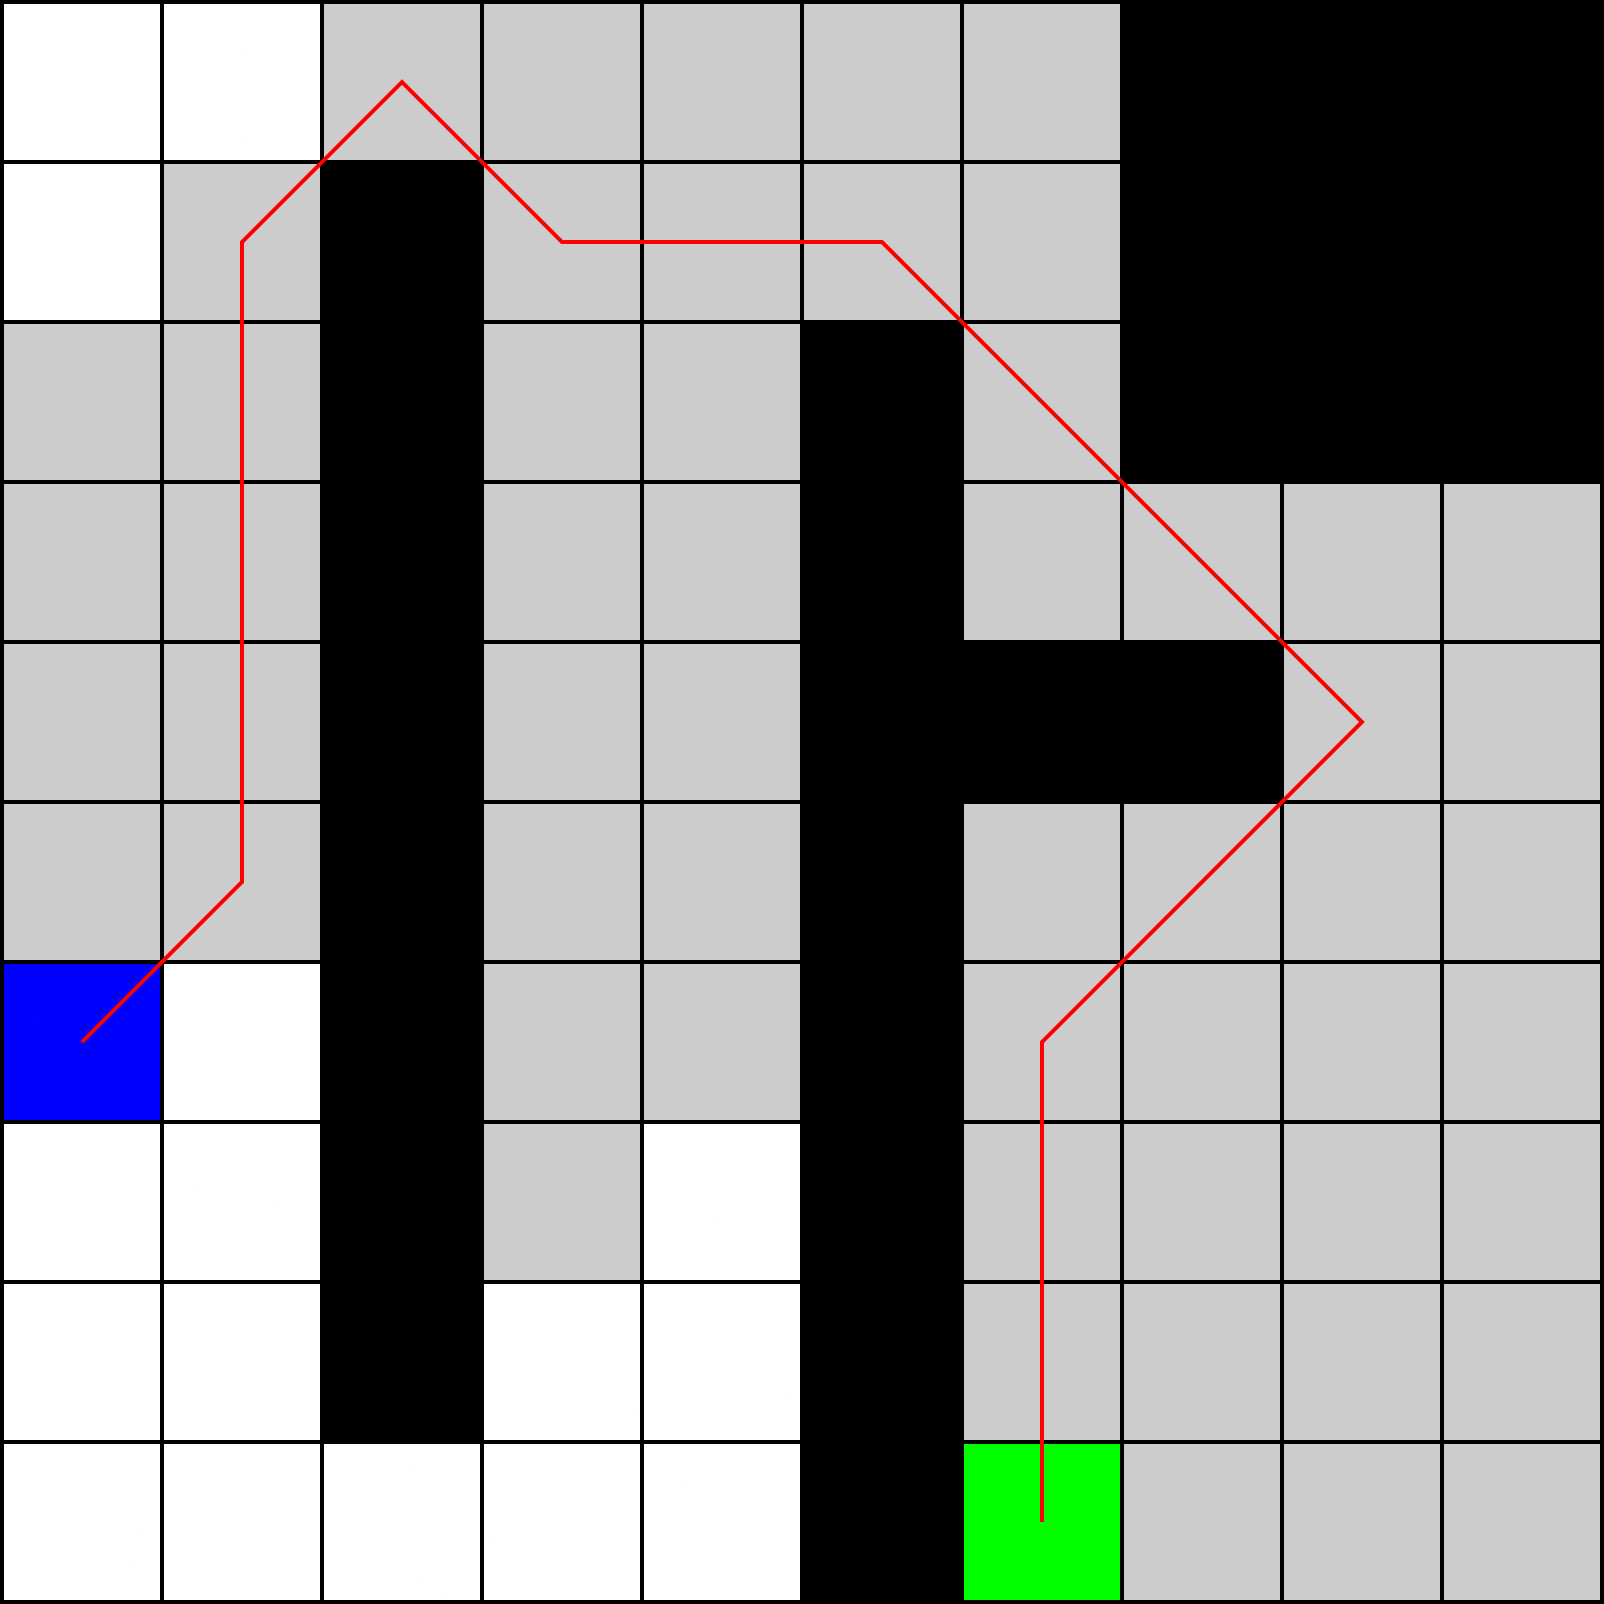
\includegraphics[width=0.45\linewidth]{images/sb.png}
            \caption{Search Based Planning Algorithms}
        \end{figure}
        These algorithms reframe the problem as a graph on the map. 
        This planning approach is optimal and offers the advantages of finding the optimal solution, enabling cost assignment, employing heuristics, and determining solution existence (completeness). 
        However, it incurs a high computational cost.
    \item Random Sampling Algorithms (PRM). 
        \begin{figure}[H]
            \centering
            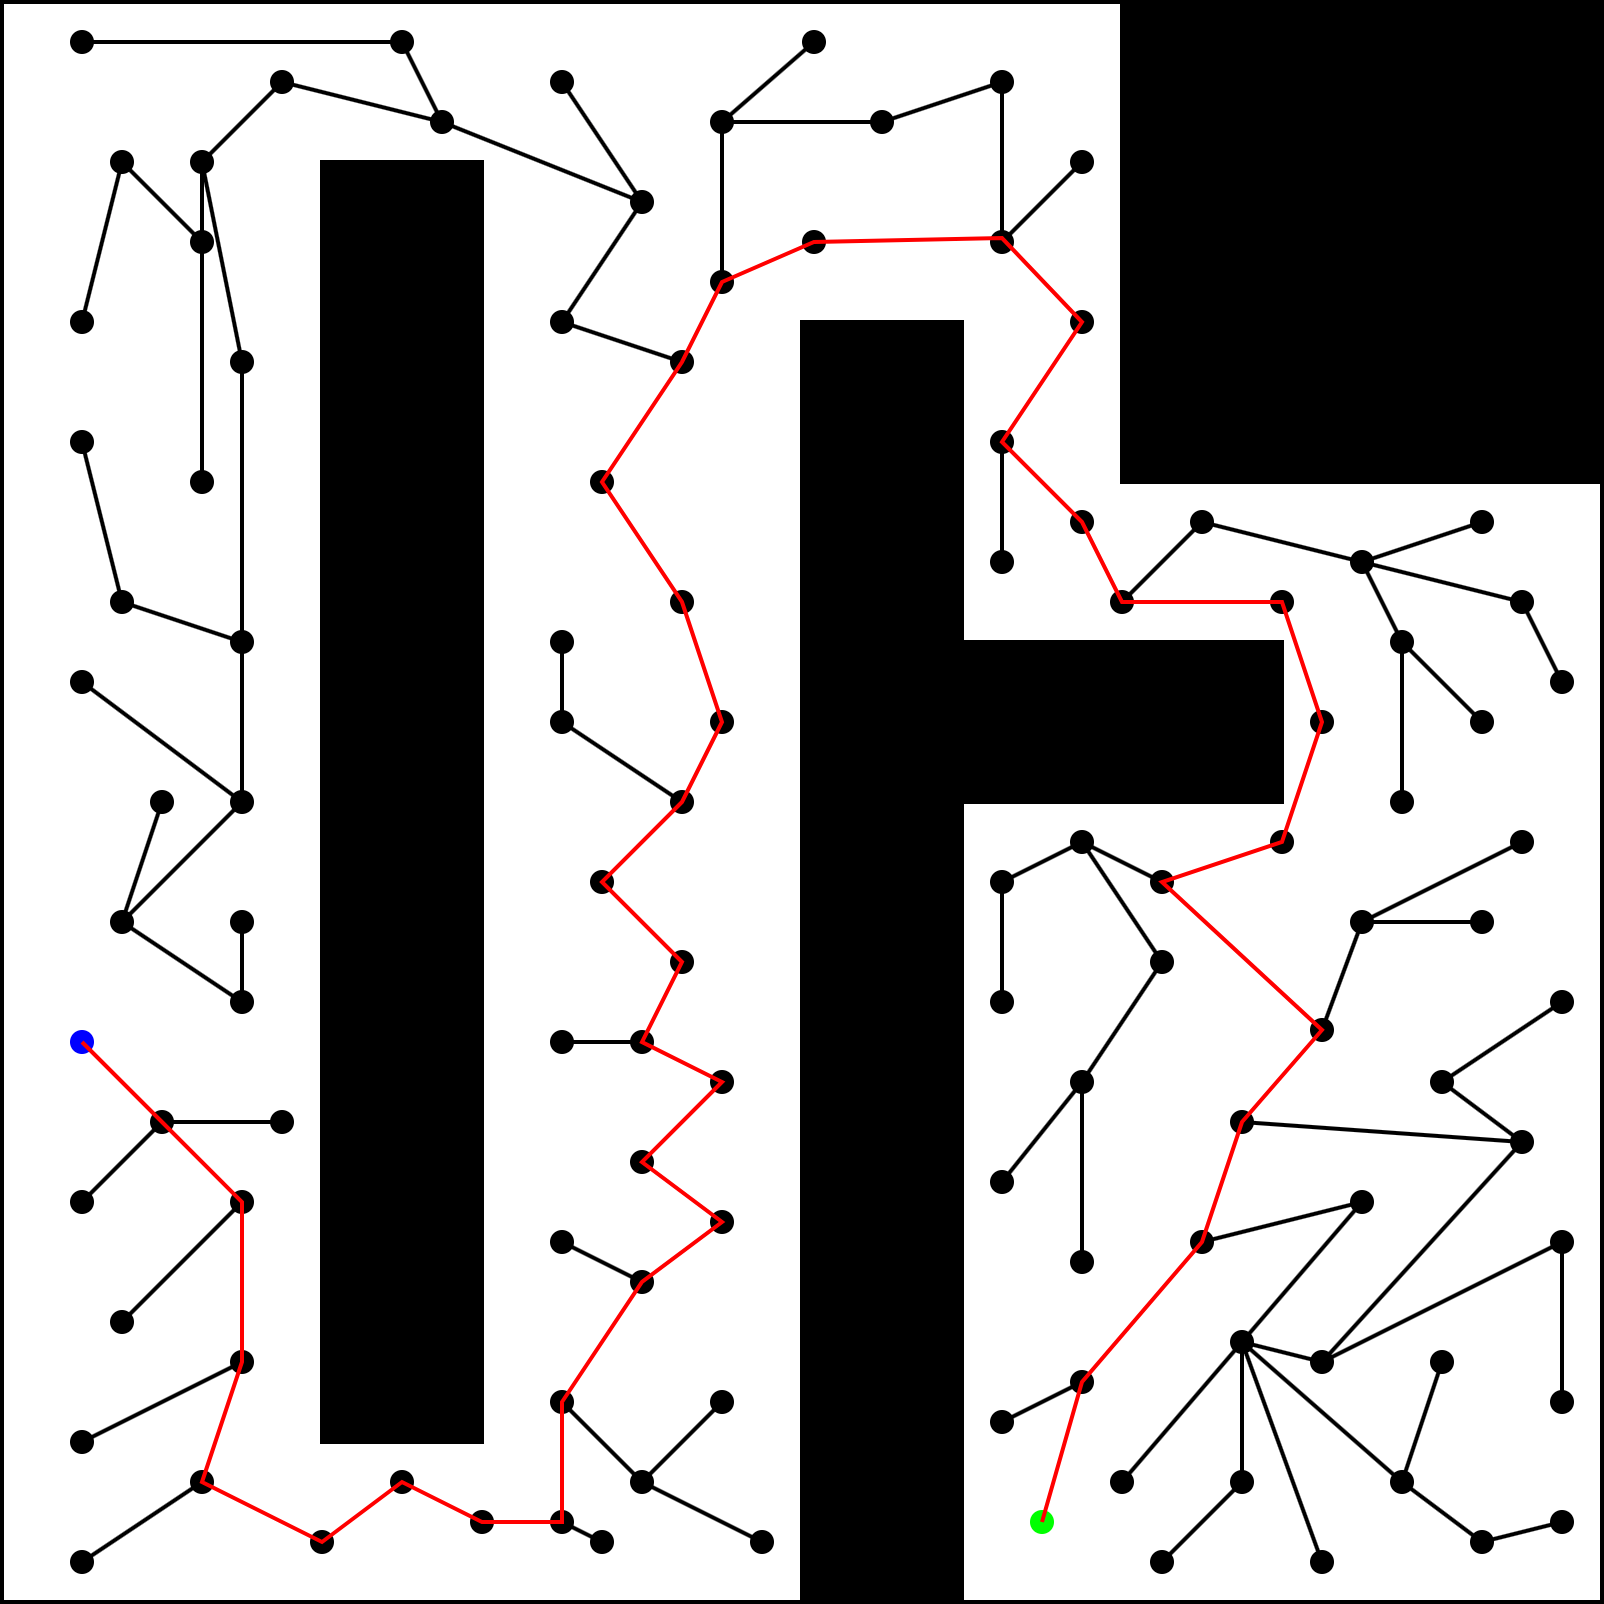
\includegraphics[width=0.45\linewidth]{images/sb1.png}
            \caption{Random Sampling Algorithms}
        \end{figure}
        Instead of using a graph, these algorithms generate a set of samples in the environment and connect them. 
        They excel in quickly finding feasible solutions.
        However, they face challenges in cost assignment and may only be probably complete, lacking a definitive way to test for solution existence.
\end{itemize}